% #############################################################################
% This is Chapter 3
% !TEX root = ../main.tex
% #############################################################################
% Change the Name of the Chapter i the following line
\fancychapter{Related Work}
\cleardoublepage
% The following line allows to ref this chapter
\label{chap:architecture}

This section reviews the datasets and architectural developments that underpin aerial image understanding, with emphasis on instance and semantic segmentation resources, referring expression segmentation datasets, historical imagery, and architectures tailored to remote sensing.

% #############################################################################
\section{Aerial Imagery Datasets}

Reliable progress in aerial image understanding depends on datasets that capture both discrete objects (e.g., ships, vehicles) and continuous land cover (e.g., roads, water, vegetation), as well as datasets that test language-based selection of specific targets. This section first summarizes instance and semantic segmentation resources that established pixel-level ground truth, and then discusses the emergence of referring expression segmentation datasets that couple images, masks, and natural language.

\subsection{Instance and Semantic Segmentation}

The iSAID dataset~\cite{zamir2019isaid} established the foundation for instance segmentation in aerial imagery by providing 655,451 object instances across 15 categories in 2,806 high-resolution images. Building upon the DOTA dataset~\cite{xia2018dota}, iSAID addressed the unique challenges of aerial imagery including high object density, large scale variations, and arbitrary orientations. The dataset demonstrated that existing computer vision methods require specialized adaptation for aerial domains, as off-the-shelf approaches achieved suboptimal performance. Example annotations are shown in Figure~\ref{fig:isaid_examples}. Key characteristics are summarized in Table~\ref{tab:source_comparison}.

\begin{figure}[t]
\centering
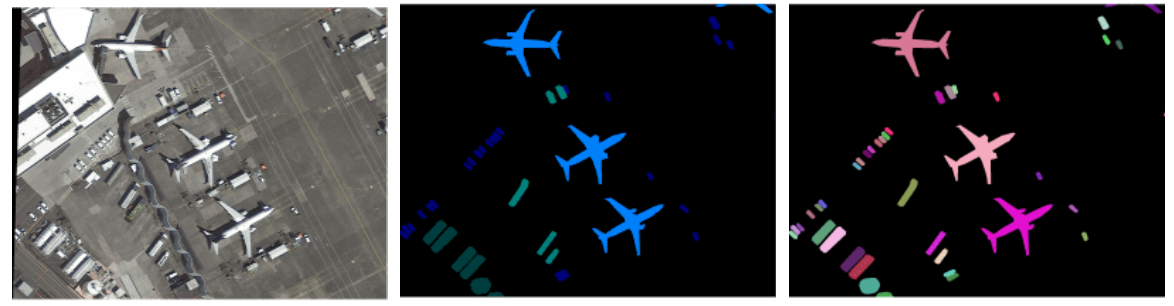
\includegraphics[width=0.8\textwidth]{Images/isaid_examples.png}
\caption{iSAID dataset examples showing instance segmentation annotations for aerial imagery, demonstrating the detailed object-level boundaries across diverse geographical contexts.}
\label{fig:isaid_examples}
\end{figure}

Complementing instance-level analysis, the LoveDA dataset~\cite{wang2021loveda} focused on land-cover semantic segmentation across urban and rural environments. Covering 536.15 km² with 0.3m resolution imagery, LoveDA enables domain adaptation research by addressing style differences between geographical environments, with urban scenes dominated by artificial objects and rural scenes containing natural elements. Representative samples appear in Figure~\ref{fig:loveda_examples}.

\begin{figure}[t]
\centering
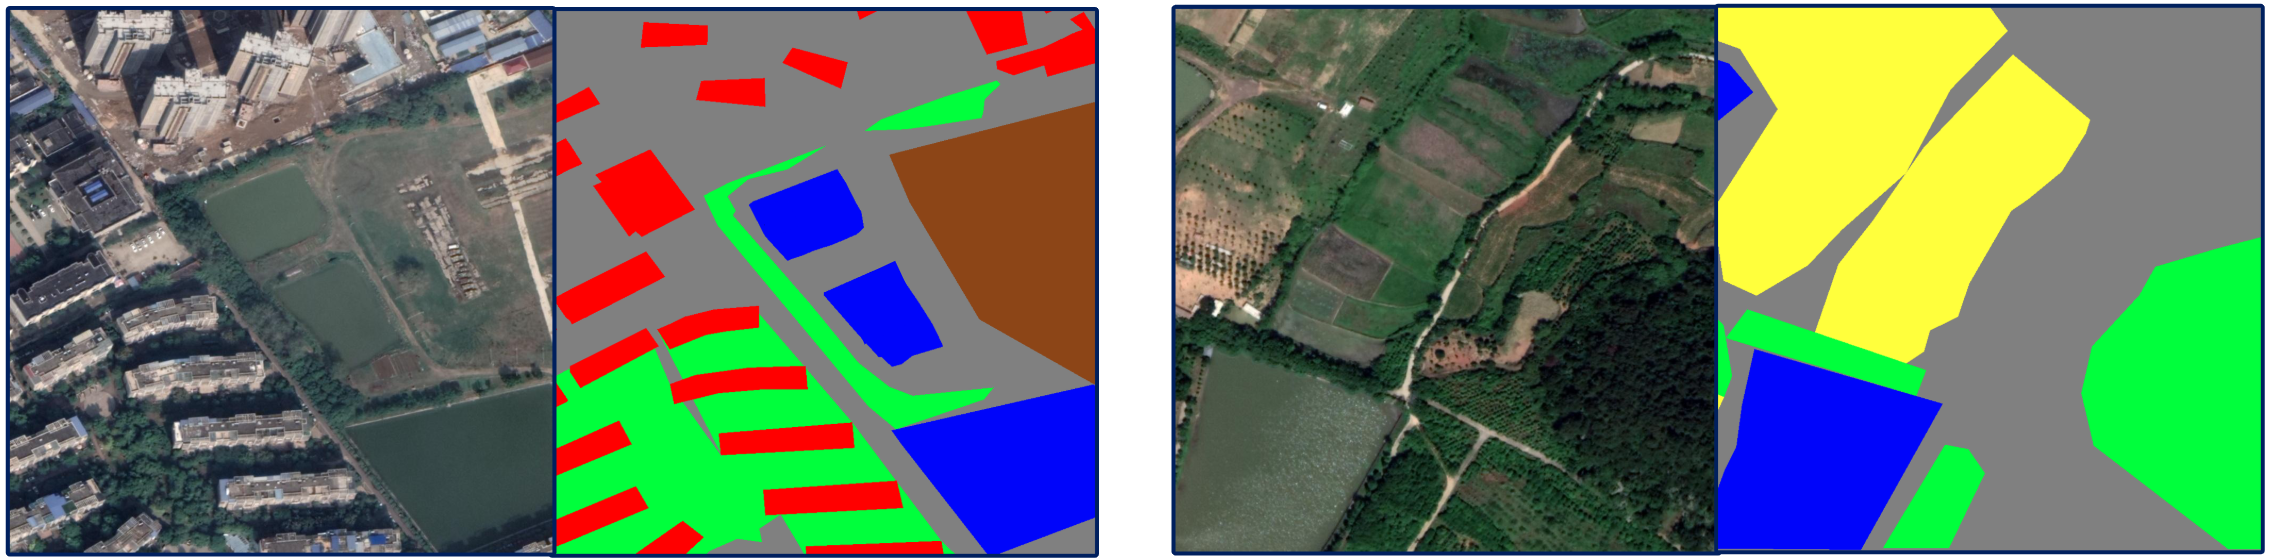
\includegraphics[width=0.8\textwidth]{Images/loveda.png}
\caption{LoveDA dataset examples showing semantic segmentation annotations for land use and land cover classification, highlighting the dense pixel-level labeling approach across urban and rural contexts.}
\label{fig:loveda_examples}
\end{figure}

\subsection{Referring Expression Segmentation Datasets}

While instance and semantic segmentation establish pixel-accurate supervision, they assume a fixed label set. Referring expression segmentation reframes the problem: given a natural language phrase, the goal is to select and segment the specific object (or group) described. In aerial imagery, this line of work began with RefSegRS~\cite{yuan2023rrsis}, which introduced 4,420 image–language–mask triplets and formalized Referring Remote Sensing Instance Segmentation (RRSIS). The dataset highlighted aerial-specific challenges—small, densely packed targets and cluttered layouts—where language can disambiguate between visually similar instances. Example samples are illustrated in Figure~\ref{fig:aerial_datasets}.

RRSIS-D~\cite{liu2024rotated} expanded both scale and annotation efficiency with 17,402 image–caption–mask triplets generated through a semi-automated pipeline using the Segment Anything Model (SAM)~\cite{sam}. The imagery originates from the DIOR dataset, grounding RRSIS-D in a broad remote-sensing corpus while leveraging automated mask generation. Beyond size, it targets aerial-specific phenomena—broad spatial scales and diverse object orientations—across 20 categories and seven attribute dimensions, enabling richer evaluation of language-guided selection in overhead scenes. Visual examples appear in Figure~\ref{fig:aerial_datasets}.

\begin{figure}[t]
\centering
\subfigure[RefSegRS dataset example samples.]{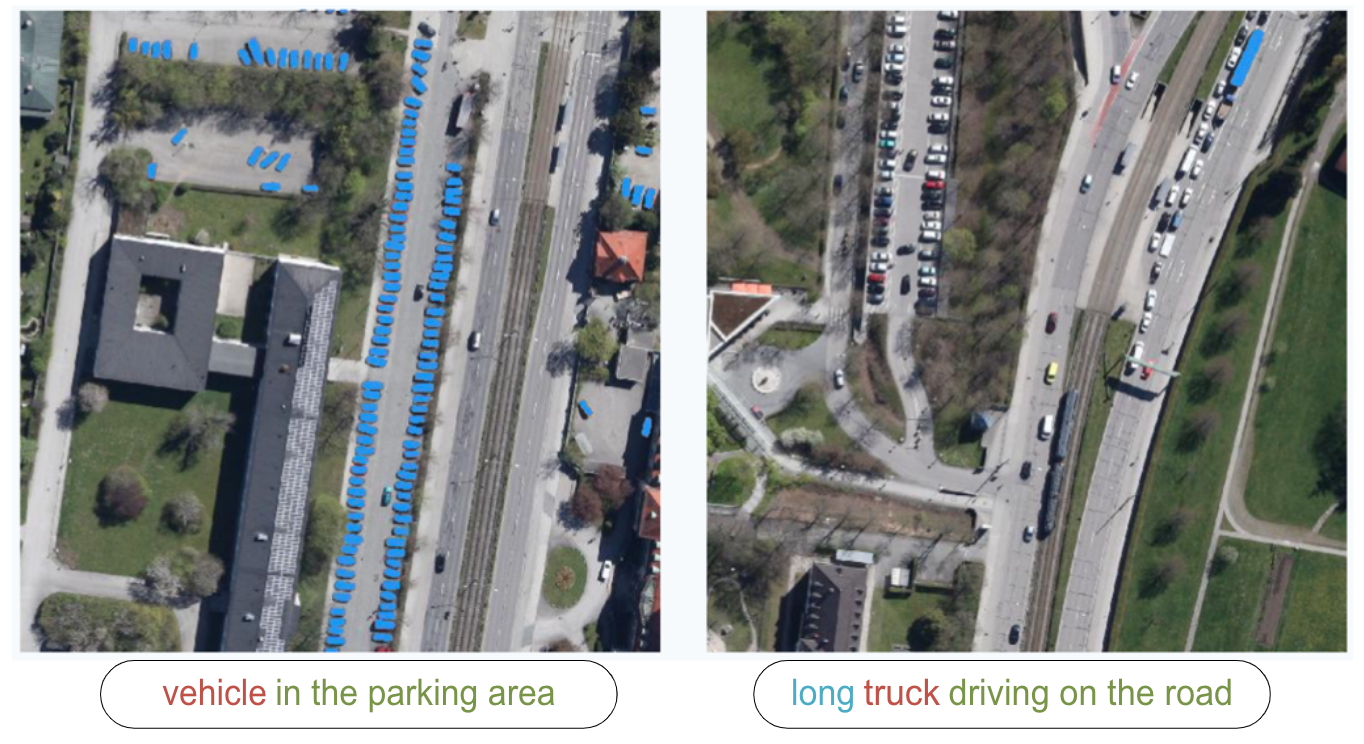
\includegraphics[width=0.45\textwidth]{Images/refsegrs.png}\label{fig:refsegrs}}
\hfill
\subfigure[RRSIS-D dataset example samples.]{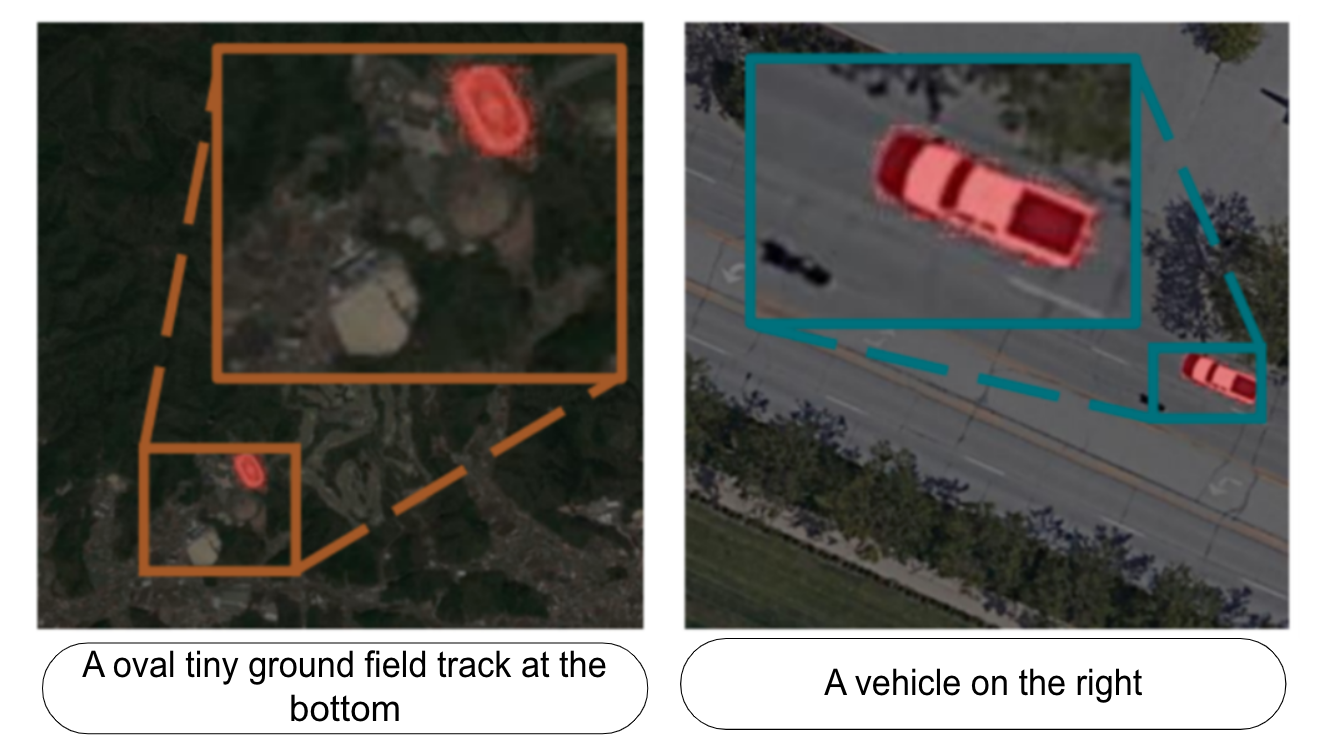
\includegraphics[width=0.45\textwidth]{Images/rrsisd.png}\label{fig:rrsisd}}
\caption{Examples from early aerial referring segmentation datasets showing the evolution from basic referring expressions to more diverse and comprehensive annotation approaches.}
\label{fig:aerial_datasets}
\end{figure}

NWPU-Refer~\cite{yang2024large} further broadens coverage with 15,003 high-resolution images and 49,745 annotated targets spanning more than 30 countries. In contrast to semi-automated pipelines, it emphasizes purely manual annotation quality and explicitly supports single-object, multi-object, and non-object scenarios across 32 categories. Together, these datasets trace a steady shift from fixed-category segmentation toward language-conditioned, fine-grained selection in aerial imagery. Comparative statistics across all referring expression segmentation datasets are presented in Table~\ref{tab:rrsis_comparison}.

\subsection{Historical Imagery Applications}

Analysing historical aerial photographs introduces practical complications—reduced contrast, grayscale capture, film artifacts, and geometric distortions—yet these datasets are vital for studying long-term urban change. Urban1960SatSeg~\cite{hao2025urban1960satseg} addresses this gap with professionally annotated semantic segmentation over 1,240 km² of declassified mid-20th-century imagery from Xi'an, China. By focusing on degraded visual conditions, it provides a reference point for methods that must remain robust when applied to archival aerial data. Representative imagery appears in Figure~\ref{fig:historical_examples}, and dataset characteristics are summarized in Table~\ref{tab:historic_comparison}.

\begin{table}[t]
\centering
\caption{Historical Imagery Dataset Summary}
\label{tab:historic_comparison}
\begin{tabular}{@{}ll@{}}
\toprule
\textbf{Feature} & \textbf{Urban1960SatSeg} \\
\midrule
Size & N/A \\
Source & 1960s urban aerial imagery \\
Annotation & Semantic segmentation (historical scenes) \\
Resolution & Variable \\
Focus & Historic urban land-cover segmentation \\
Categories & Buildings, roads, vegetation, open spaces \\
\bottomrule
\end{tabular}
\end{table}

\begin{figure}[t]
\centering
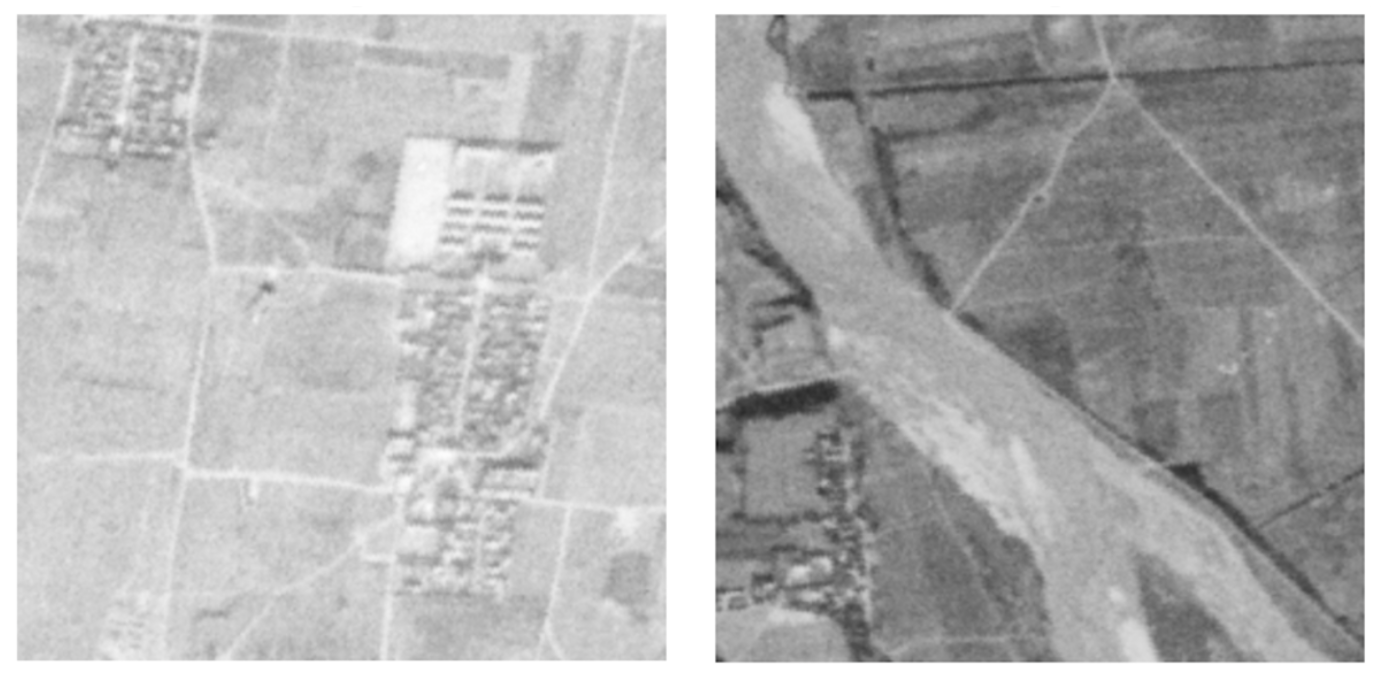
\includegraphics[width=0.6\textwidth]{Images/1960.png}
\caption{Historical aerial imagery examples from the UrbanSatSeg1960 dataset showing the characteristic visual properties of 1960s aerial photography, including reduced contrast, grayscale capture, and period-specific urban development patterns.}
\label{fig:historical_examples}
\end{figure}

\begin{table}[t]
\centering
\caption{Source Aerial Dataset Comparison}
\label{tab:source_comparison}
\begin{tabular}{@{}lll@{}}
\toprule
\textbf{Feature} & \textbf{iSAID} & \textbf{LoveDA} \\
\midrule
Size & 655,451 instances & 5,987 images \\
Source & DOTA (re-ann.) & Spaceborne (0.3m) \\
Annotation & Professional & Manual \\
Resolution & High res. & 1024×1024px \\
Focus & Instance Seg. & Land-cover Seg. + UDA \\
Categories & 15 & 7 \\
Attributes & - & Domain labels \\
\bottomrule
\end{tabular}
\end{table}

\begin{table}[t]
\centering
\caption{Aerial Referring Segmentation (RRSIS) Dataset Comparison}
\label{tab:rrsis_comparison}
\begin{tabular}{@{}llll@{}}
\toprule
\textbf{Feature} & \textbf{RefSegRS} & \textbf{RRSIS-D} & \textbf{NWPU-Refer} \\
\midrule
Size & 4,420 triplets & 17,402 triplets & 49,745 triplets \\
Source & SkyScapes & RSVGD & Multi-source global \\
Annotation & Manual & Semi-auto (SAM) & Manual \\
Resolution & Limited & 800×800 fixed & 1024-2048px \\
Focus & RRSIS & RRSIS & RRSIS \\
Categories & - & 20 & 32 \\
Attributes & 3 & 7 & 6 dimensions \\
\bottomrule
\end{tabular}
\end{table}


% #############################################################################
\section{Architectures for RRSIS}

Architectures for referring expression segmentation in aerial imagery combine vision backbones, language encoders, and fusion mechanisms that translate textual cues into pixel-level masks. The Rotated Multi-Scale Interaction Network (RMSIN)~\cite{liu2024rotated} is a representative design that builds bespoke processing blocks on top of a Swin Transformer visual encoder and a BERT language backbone. Its Intra-scale Interaction module refines fine-grained details with transformer blocks, the Cross-scale Interaction module aligns multi-resolution features through cross-attention, and the Adaptive Rotated Convolution module injects rotation-aware convolutional filters to handle arbitrary object orientations.

MRSNet~\cite{yang2024large} adopts the same Swin–BERT backbone pairing but alters how features interact. Instead of RMSIN's triplet of modules, it employs hierarchical fusion that first consolidates information within each scale before exchanging context across scales, leading to a more progressive flow of visual detail toward the mask decoder. The shift in interaction pattern highlights how architectural variants largely differ in their feature fusion strategies rather than wholesale backbone changes.

RSRefSeg~\cite{chen2025rsrefseg} illustrates the alternative of leaning fully on large vision–language models. It replaces bespoke encoders with CLIP~\cite{clip} or SigLIP~\cite{siglip} for multimodal feature extraction and integrates SAM~\cite{sam} as the segmentation decoder. A lightweight AttnPrompter module converts language-conditioned features into sparse and dense prompts for SAM, while LoRA adapters~\cite{lora} fine-tune both CLIP/SigLIP and the SAM vision encoder to aerial imagery. Figure~\ref{fig:rsrefseg_architecture} visualizes this configuration and highlights how the prompts interface with SAM. This design achieves the strongest reported IoU on RRSIS-D~\cite{liu2024rotated,chen2025rsrefseg} while requiring updates only to the bridging layers and low-rank adapters.

\begin{figure*}[t]
\centering
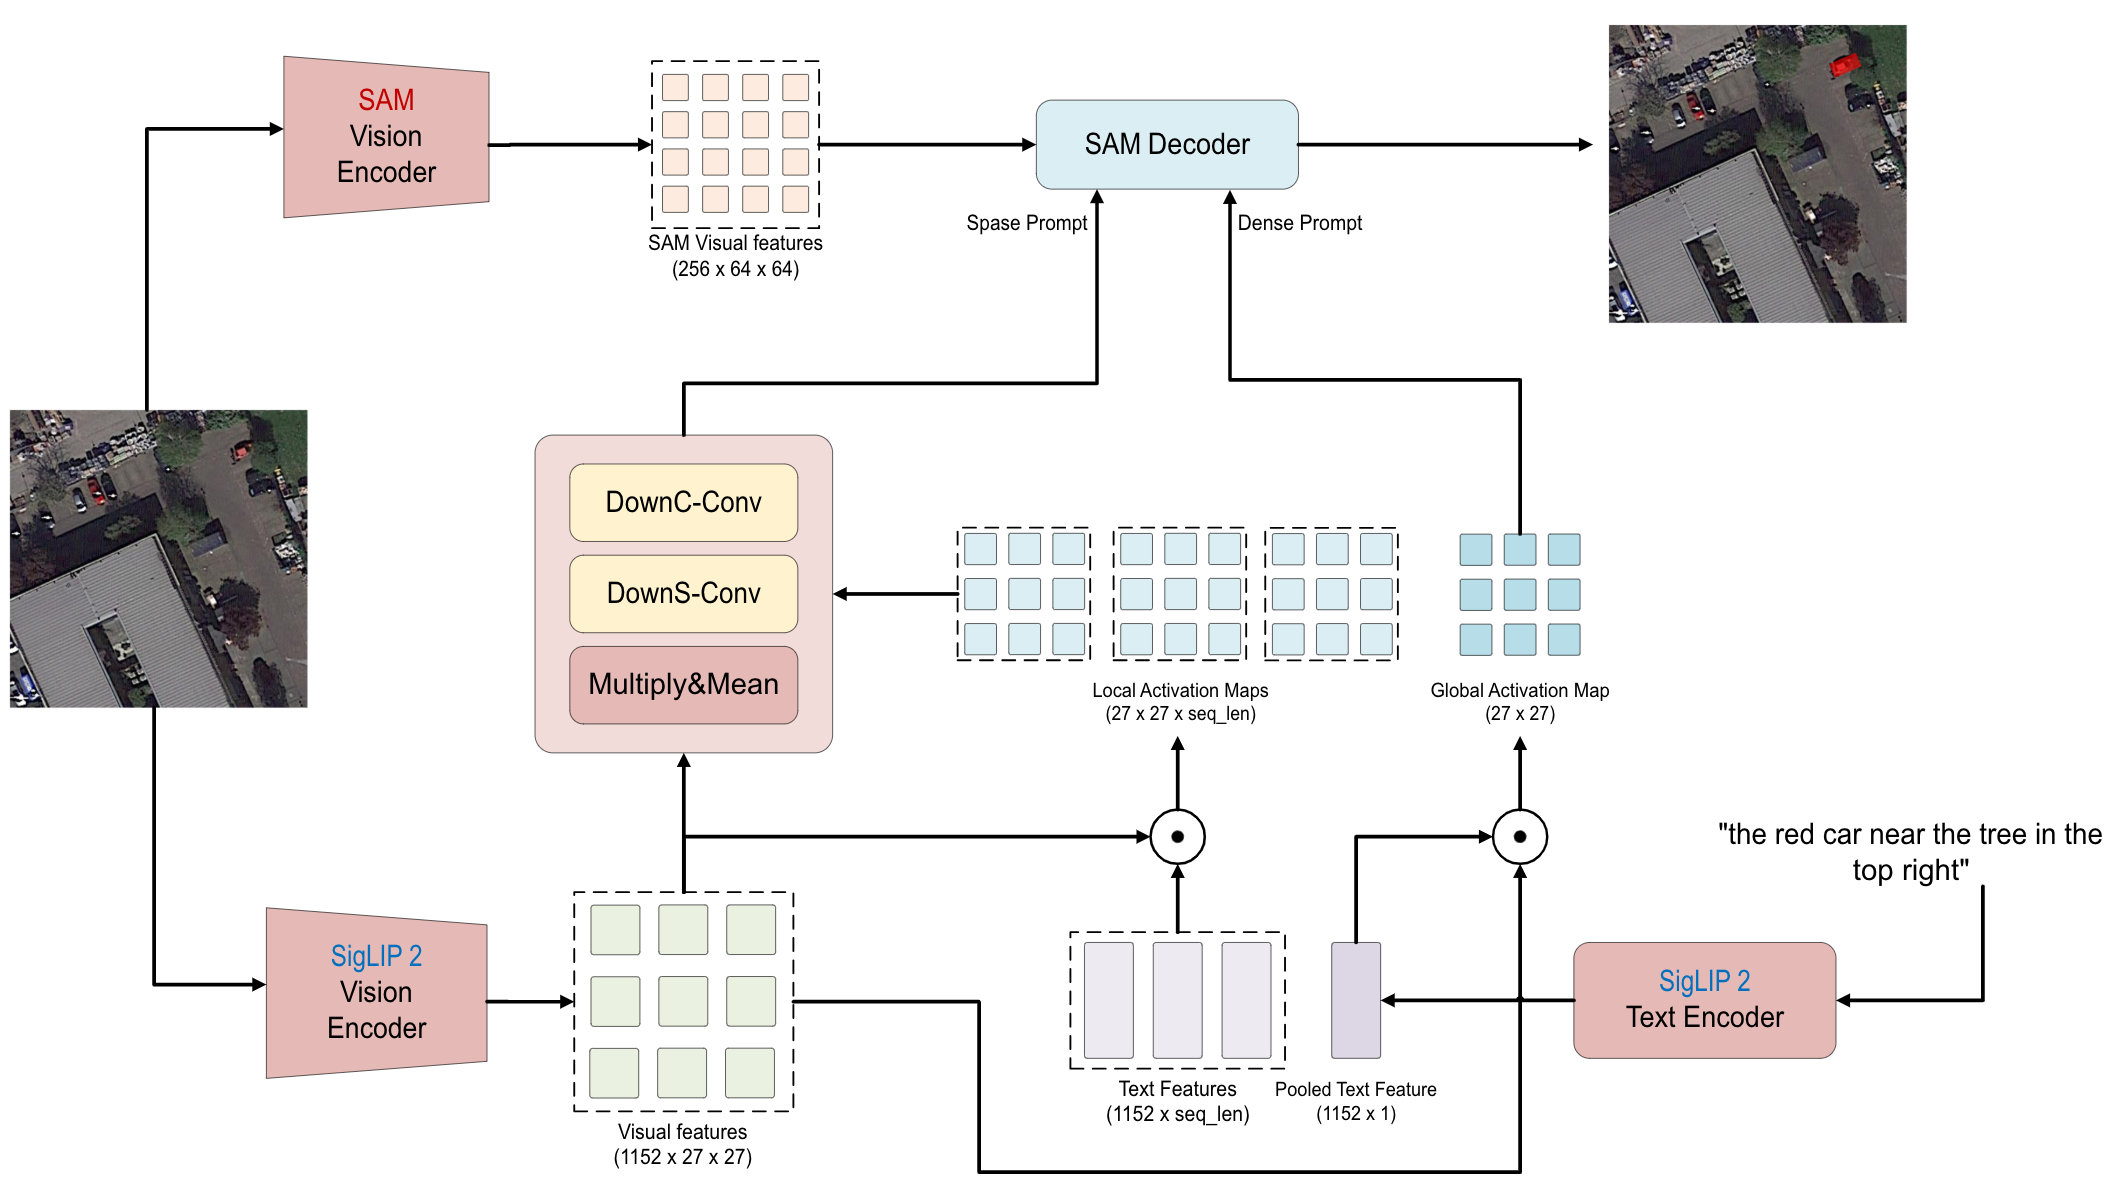
\includegraphics[width=0.9\textwidth]{Images/clipsam.png}
\caption{Overview of the RSRefSeg architecture~\cite{chen2025rsrefseg}, which couples a vision–language encoder with a segmentation decoder via a learned prompting bridge.}
\label{fig:rsrefseg_architecture}
\end{figure*}

% #############################################################################
\section{Overview}

The current landscape of aerial image segmentation is shaped by three pillars that enable language-guided segmentation. First, instance and semantic datasets such as iSAID and LoveDA supply pixel-accurate supervision for objects and land cover. Second, referring expression segmentation datasets including RefSegRS, RRSIS-D, and NWPU-Refer pair images with natural expressions and masks, enabling evaluation of language-conditioned target selection at varying scales and annotation regimes. Third, architectural developments span specialized remote-sensing networks (e.g., RMSIN, MRSNet) and foundation-model designs (e.g., RSRefSeg~\cite{chen2025rsrefseg}) that leverage strong vision and language backbones.

Crucially, the complementary supervision in iSAID and LoveDA presents an opportunity to construct a larger and more diverse referring expression segmentation resource by converting instance- and land-cover annotations into language-conditioned targets—motivating the creation of Aerial-D as a comprehensive dataset for aerial referring expressions.

Within this context, RSRefSeg stands out as a particularly compelling choice for referring expression segmentation: it benefits from powerful pretrained vision–language encoders (e.g., CLIP/SigLIP) and a high-capacity segmentation decoder (SAM) connected by a lightweight bridging mechanism. The resulting system establishes the leading IoU on RRSIS-D~\cite{chen2025rsrefseg}, demonstrating that foundation-model backbones can be adapted effectively to aerial referring expression segmentation.